\section{Results}\label{sec:results}
All results use the CFRP lamina of Sec.~\ref{sec:model} unless stated, an $x$-directed drive
at the left edge (a plane-wave line source for the lens and the cloak, a Gaussian beam for
the panel, Table~\ref{tab:panelparams}), and the absorbing sponge on the other three
sides. Only the
fiber orientation is designed. Material, thickness and mass are identical to the
straight-fiber baseline.

\subsection{The lens: what the optimizer buys, and what it does not (W1, W2)}\label{sec:lens}
On a $4\times3$ plate at $\omega=40$ (Table~\ref{tab:params}), maximizing the energy in
a target box (dashed square in Fig.~\ref{fig:lens}) yields a mirror-symmetric field of
tows bending toward the target near the right end of the plate. The single-frequency target-energy gain against straight
fibers is $G=\WGainForty\times$. The decomposition \eqref{eq:gainsplit} shows what this
number contains (Fig.~\ref{fig:lensband}, Table~\ref{tab:lensband}).
\begin{itemize}[itemsep=1pt]
\item \textbf{Redirection.} The target's share of the interior energy rises from
  $\WPhiZero\%$ to $\WPhiOne\%$, a redirection $G_\varphi=\WRedirForty\times$.
\item \textbf{Field growth.} The whole interior field grows $\WGrowthForty\times$.
\item \textbf{Source power.} The design draws $\WPowerForty\times$ more power from the
  force source.
\end{itemize}
Sweeping the drive frequency on the \emph{fixed} design separates the two factors as W2
predicts. The redirection is broadband once the wavelength is short against the lens:
$G_\varphi\ge\WRedirBandMin\times$ for every $\omega\in[37.5,60]$, and the band average
$\langle G_\varphi\rangle_{\rm band}$, defined throughout as the mean of $G_\varphi$ at
$\omega\in\{35,40,45,50\}$, is $\WRedirBandMean\times$. At $\omega=20$ and $25$ the redirection
collapses and even reverses ($G_\varphi<1$, Table~\ref{tab:lensband}): there the
along-fiber wavelength exceeds the length over which the fiber field turns, and the ray
picture of Sec.~\ref{sec:theory} no longer applies. These values depend on the absorbing
layer: with one reflecting $|R|\le\WReflThickMax$ instead of $\WReflMin$--$\WReflMax$, the lens re-optimized from scratch gives
$G=\WAbsG\times$ at $\omega=40$, split into $G_\varphi=\WAbsP\times$ and $\WAbsGr\times$
growth, and $G_\varphi\ge\WAbsMinFortySixty\times$ over $[40,60]$ ($\WAbsThirtySevenFive\times$
at $37.5$), band average $\WAbsBand\times$ (Appendix~\ref{app:verify}). The split, and the
resonant nature of the excess gain, are unchanged. The
field growth is a resonance of the finite plate at the design frequency. At $\omega=37.5$
and $42.5$, only $\pm6\%$ away, $G$ falls to $\WGainMinusFive\times$ and
$\WGainPlusFive\times$, while $G_\varphi$ changes far less (from
$\WRedirForty$ to $\WRedirBandMin$--$6.1$). A large single-frequency
focus gain is therefore not by itself evidence of steering. It mostly measures how well
the optimizer tuned a standing wave. The physical, transferable result is the
redirection.

For W1, setting the lamina isotropic makes $G=G_\varphi=1$ to machine precision, and
every orientation gradient vanishes identically (Remark~\ref{rem:iso};
Sec.~\ref{sec:dose}).

\begin{table}[h]
\centering\small
\caption{The lens design (optimized at $\omega=40$) evaluated across frequency. $G$:
target-energy gain; $G_\varphi$: redirection (target share of interior energy, relative to
straight fibers); growth: interior energy ratio; $P$: injected power ratio. $G=G_\varphi
\times$growth exactly.}
\label{tab:lensband}
\IfFileExists{wt_lensband_table.tex}{\begin{tabular}{@{}rrrrr@{}}
\toprule
$\omega$ & $G$ & $G_\varphi$ & growth & $P/P_0$\\ \midrule
20.0 & 0.2 & 0.25 & 0.74 & 0.61\\
25.0 & 0.9 & 0.41 & 2.26 & 0.96\\
30.0 & 3.7 & 1.65 & 2.25 & 0.92\\
35.0 & 2.1 & 2.34 & 0.89 & 0.49\\
37.5 & 6.6 & 3.74 & 1.77 & 0.80\\
\bf 40.0 & \bf 78.0 & \bf 5.82 & \bf 13.41 & \bf 4.13\\
42.5 & 10.1 & 6.10 & 1.65 & 0.95\\
45.0 & 16.3 & 6.54 & 2.49 & 1.28\\
50.0 & 5.5 & 6.01 & 0.91 & 0.70\\
55.0 & 5.7 & 4.27 & 1.34 & 0.91\\
60.0 & 5.8 & 3.71 & 1.58 & 1.08\\
\bottomrule
\end{tabular}
}{\textit{(pending: run in progress)}}
\end{table}

\begin{figure}[h]
\centering
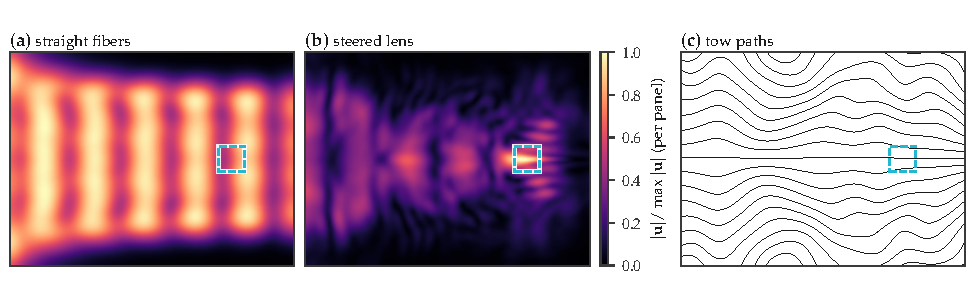
\includegraphics[width=\textwidth]{figs/wt_lens.pdf}
\caption{The orientation-only lens at its design frequency ($\omega=40$), on the full
$4\times3$ plate driven at its left edge. \textbf{(a)}~Field
magnitude $|\vu|$ with straight fibers, and \textbf{(b)}~with the optimized fiber field; each map
is normalized by its own maximum, so the comparison is of \emph{where} the energy goes (the
absolute ratio is the gain $G$); dashed square: the objective region
$(0.78L_x,L_y/2)\pm0.18$. \textbf{(c)}~Optimized tow paths
(mirror-symmetric, bending toward the objective region near the right end). The $\WGainForty\times$ focus gain of (b) over
(a) is $\WRedirForty\times$ redirection times a resonant field growth
(Sec.~\ref{sec:lens}).}
\label{fig:lens}
\end{figure}

\begin{figure}[h]
\centering
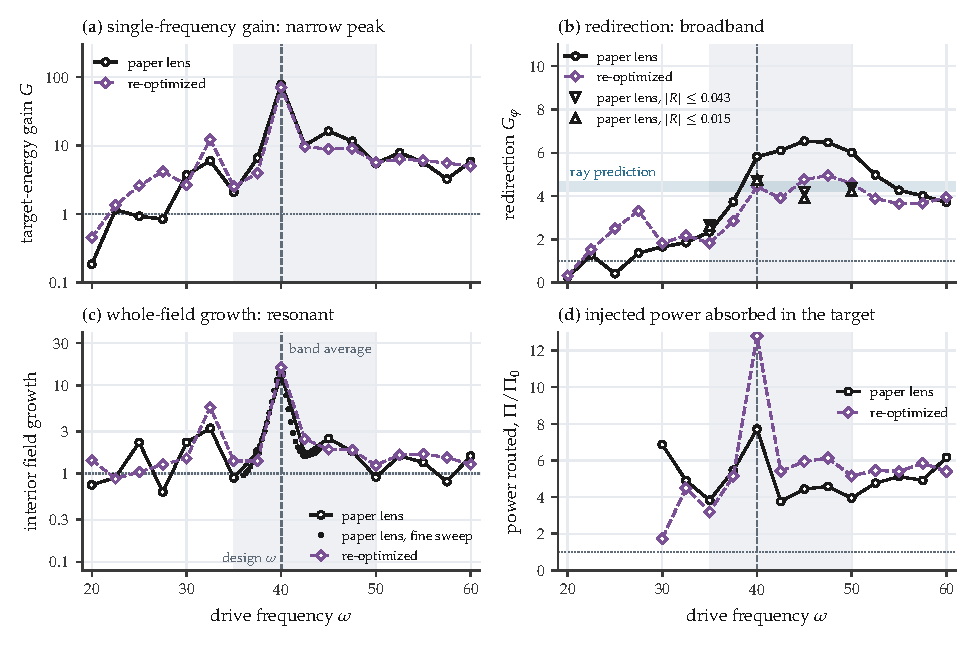
\includegraphics[width=\textwidth]{figs/wt_lens_band.pdf}
\caption{What the lens does across frequency (design fixed, optimized at $\omega=40$).
\textbf{(a)}~Single-frequency gain $G$ (log scale) and its two factors: redirection
$G_\varphi$ (broadband) and interior field growth (resonant); dotted: parity with straight
fibers. \textbf{(b)}~Target share of interior energy, straight vs.\ steered: the steered
plate sends at least $\WRedirBandMin\times$ more of its energy to the target at every
frequency in $\omega\in[37.5,60]$.}
\label{fig:lensband}
\end{figure}

\subsection{Mechanism: the energy flux follows the fibers (W3)}\label{sec:flux}
We compute the time-averaged elastic energy flux of the solved field cell by cell,
$P_j=-\tfrac12\Real\{\sigma_{ij}\bar v_i\}=\tfrac{\omega}{2}\big[\sigma_{ij}(\vu^{\rm r})\,u^{\rm i}_i-\sigma_{ij}(\vu^{\rm i})\,u^{\rm r}_i\big]$ (for $e^{+\ii\omega t}$, $\bm v=\ii\omega\vu$), and
measure its angle to the local fiber director (Fig.~\ref{fig:flux}).
\begin{itemize}[itemsep=1pt]
\item \textbf{Optimized lens.} The $|\bm P|$-weighted mean deviation of the flux from the
  fibers is $\WFluxDev^\circ$, and $\WFluxShare\%$ of the energy flux runs within
  $20^\circ$ of them. The flux deviates $\WFluxDevX^\circ$ on average from the drive
  direction $x$.
\item \textbf{Across the band.} At $\omega=35,45,50$ the flux--fiber deviation is
  $\WFluxDevThirtyFive^\circ$, $\WFluxDevFortyFive^\circ$ and $\WFluxDevFifty^\circ$.
\item \textbf{Control: fields that were never optimized.} Three random smooth CS-RBF fields
  (same support grid as the lens, support values drawn from $\mathcal N(0,0.5\,\mathrm{rad})$)
  and one analytic field, $\theta=0.6\sin(\pi x/2)\sin(2\pi y/3)$, give flux--fiber
  deviations of only $\WCtrlDevMin$--$\WCtrlDevMax^\circ$ at $\omega=40$ and $50$, against
  $\WCtrlXMin$--$\WCtrlXMax^\circ$ from the drive direction
  (Appendix~\ref{app:verify}). Their fields turn more gently than the lens's, which
  is why they channel even more tightly.
\end{itemize}
The energy goes where the fibers point, at every frequency tested and whether or not the
field was optimized: channeling is imposed by the lamina, and the optimizer only chooses
where the fibers point. This is the channeling
predicted by \eqref{eq:skew}, and it is why the redirection is broadband.

\begin{figure}[h]
\centering
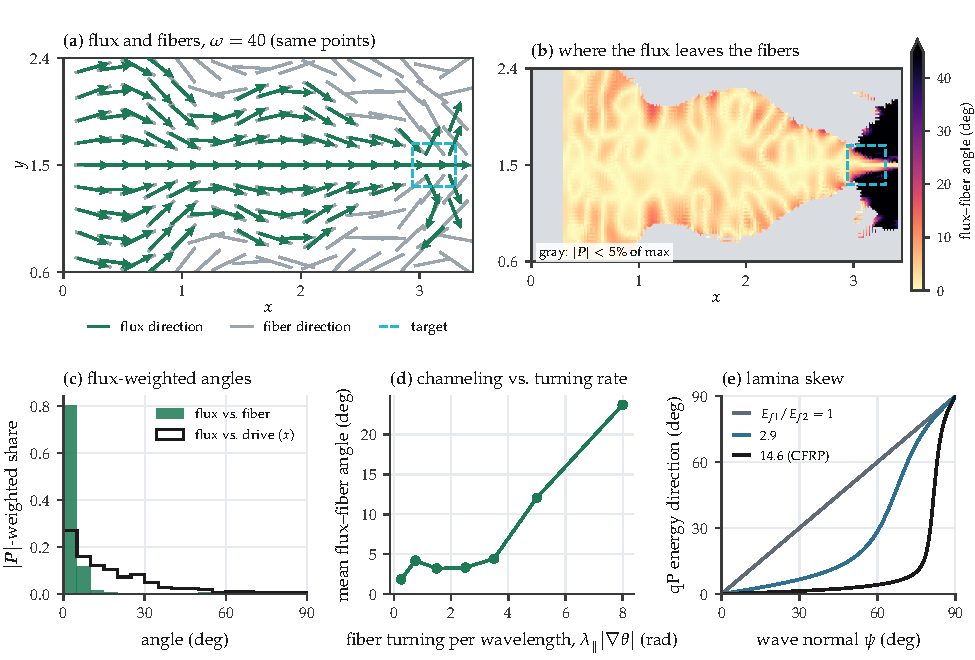
\includegraphics[width=\textwidth]{figs/wt_flux.pdf}
\caption{Energy channeling. \textbf{(a)}~Time-averaged energy-flux streamlines of the
optimized lens at $\omega=40$ over the fiber director field (gray dashes), in
the window $0\le x\le3.4$, $0.6\le y\le2.4$ that excludes the absorbing layers; dashed
square: objective region. \textbf{(b)}~The
$|\bm P|$-weighted distribution of the angle between the flux and the local fiber, and
between the flux and the drive direction. \textbf{(c)}~The qP energy direction vs.\ wave
normal \eqref{eq:skew} for an isotropic lamina (diagonal: no skew), the intermediate
lamina $E_{f1}/E_{f2}=2.9$ of the family $\mathbf Q(s)$, and CFRP ($E_{f1}/E_{f2}=14.6$): in CFRP most normals
carry their energy close to the fiber.}
\label{fig:flux}
\end{figure}

\subsection{How the control scales with anisotropy (W4)}\label{sec:dose}
Along the family $\mathbf Q(s)=\mathbf Q_{\rm iso}+s(\mathbf Q_f-\mathbf Q_{\rm iso})$,
which holds the isotropic invariants and scales the anisotropic ones by $s$, we
re-optimize the lens for each material (Table~\ref{tab:dose}, Fig.~\ref{fig:limitsW}a).
The band-averaged redirection does not decrease with anisotropy in these runs. It is exactly $1$ at
isotropy, rises steeply to $\WDoseThree\times$ by $E_{f1}/E_{f2}\approx3$ (where
$s_{20}$ already exceeds $60\%$), reaches $\WDoseCFRP\times$ for CFRP, and
$\WDoseMax\times$ at $E_{f1}/E_{f2}=32$. The single-frequency gain $G$ along the same
family is \emph{non-monotone} ($\WDoseGThree\times$ at $E_{f1}/E_{f2}=2.9$ but
$\WDoseGFive\times$ at $5.4$), because it is dominated by whichever resonance each
optimization happens to tune. The trend should be read coarsely: for the same CFRP problem, different
optimizer runs give a band-averaged redirection from $\WRedirBandMean\times$ (the lens of
Sec.~\ref{sec:lens}) to $\WFrontUnc\times$ (the best front design, Sec.~\ref{sec:front}),
a spread comparable to the steps between neighboring laminae. Robust are the end points
($1$ at isotropy, several times once $E_{f1}/E_{f2}\gtrsim3$), not the detailed shape,
such as the plateau between $E_{f1}/E_{f2}=2.9$ and $5.4$.

\begin{table}[h]
\centering\small
\caption{Lens re-optimized for each lamina of the anisotropy family. $s_{20}$: channeling
share (Sec.~\ref{sec:theory}).}\label{tab:dose}
\IfFileExists{wt_dose_table.tex}{\begin{tabular}{@{}ccccccc@{}}
\toprule
$s$ & $E_{f1}/E_{f2}$ & $s_{20}$ & $G(40)$ & $G_\varphi(40)$ & $\langle G_\varphi\rangle_{\rm band}$, 4 starts & better absorber, 4 starts\\ \midrule
0.00 & 1.0 & 22\% & 1.0 & 1.00 & 1.00 & 1.00\\
0.25 & 1.7 & 42\% & 6.9 & 2.63 & 1.86--1.88 & 2.68--2.71\\
0.50 & 2.9 & 60\% & 24.1 & 6.92 & 2.94--4.21 & 2.09--3.00\\
0.75 & 5.4 & 75\% & 16.2 & 5.49 & 3.59--4.62 & 2.61--3.35\\
1.00 & 14.6 & 88\% & 78.0 & 5.82 & 5.13--5.74 & 3.92--4.25\\
1.10 & 31.9 & 94\% & 162.4 & 5.85 & 6.06--6.94 & 4.46--4.95\\
\bottomrule
\end{tabular}
}{\textit{(pending: run in progress)}}
\end{table}

\subsection{Manufacturing limits (W5): tow curvature}\label{sec:front}
We bound the tow curvature $|\zeta|\le\zeta_{\rm all}=1/R$, keeping the lens's own mesh,
frequency and parametrization (Table~\ref{tab:front}, Fig.~\ref{fig:limitsW}b).
\begin{itemize}[itemsep=1pt]
\item \textbf{Plateau.} The best band-averaged redirection stays at
  $\WFrontOne$--$\WFrontUnc\times$ for every limit down to $\zeta_{\rm all}=1.0$, i.e.\ a
  minimum tow radius $R=1.0\approx0.7\lambda$, where $\lambda=1.42$ is the along-fiber qP
  wavelength at $\omega=40$ (the longest wavelength present; against the cross-fiber qP
  wavelength $0.37$ the same radius is $2.7$ wavelengths). We use the along-fiber value
  because the channeled energy travels along the fibers. The front lies at the edge of the
  slowly-turning regime assumed by the ray argument of Sec.~\ref{sec:theory}, so we read
  it as an empirical scale rather than a ray prediction.
\item \textbf{Decline.} Beyond that radius the best design found falls gradually, not
  abruptly:
  $\WFrontEight\times$ at $R=1.25$, $\WFrontSix\times$ at $R=1.67$ ($\approx1.2\lambda$),
  $\WFrontFourFive\times$ at $R=2.2$ and $\WFrontTight\times$ at $R=\WFrontTightR$. Tows that
  cannot turn on the wavelength scale cannot converge the channeled energy on the target
  within the plate.
\end{itemize}
Physically, energy can be redirected only if the tows can turn on the wavelength scale.
\paragraph{How the front is computed, and how robust it is.} The optimizations are local
and strongly start-dependent under a curvature limit. At each limit from
$\zeta_{\rm all}=0.3$ to $1.5$ we therefore run $\WFrontNStart$ starts ($\WFrontNDistinct$ of which lead to distinct designs): every
earlier front design and three random fields, each scaled until feasible
(\texttt{lens\_\allowbreak front\_\allowbreak robust.py}). The spread is large (at
$\zeta_{\rm all}=1.0$ from $\WFrontOneMin\times$ to $\WFrontOne\times$; shaded bars in
Fig.~\ref{fig:limitsW}b), so single runs can stall far below what the limit permits: an
earlier single-run front reported a collapse to $1.3\times$ at $R=1.67$, which the
multi-start study shows was a stalled run. A design whose actual curvature satisfies a
limit is feasible for that limit and for every looser one, so Table~\ref{tab:front}
reports, at each limit, the best band-averaged redirection over \emph{all} computed
designs that satisfy it; for $\zeta_{\rm all}=\infty$ every design counts, and the best
($\WFrontUnc\times$) comes from a run at $\zeta_{\rm all}=1.5$. These values are lower
bounds on what each limit allows. The best unconstrained-objective designs also redirect
more than the lens of Sec.~\ref{sec:lens} ($\WRedirBandMean\times$): the single-frequency
objective does not determine the redirection uniquely, which is another reason to report
and optimize the band-averaged quantity.

\begin{table}[h]
\centering\small
\caption{Lens manufacturability front (same mesh, frequency and parametrization as
Sec.~\ref{sec:lens}). Each row is the best band-averaged redirection over all computed
designs whose curvature satisfies the limit (a lower bound on what the limit allows); the
last column is the range over the independent starts run at that limit.}\label{tab:front}
\IfFileExists{wt_front_table.tex}{\begin{tabular}{@{}ccccccc@{}}
\toprule
$\zeta_{\rm all}$ & $R=1/\zeta_{\rm all}$ & $\max|\zeta|$ & $G(40)$ & $G_\varphi(40)$ & $\langle G_\varphi\rangle_{\rm band}$ & range over starts\\ \midrule
$\infty$ & 0 & 1.47 & 13.2 & 7.49 & 6.80 & --\\
4 & 0.25 & 1.47 & 13.2 & 7.49 & 6.80 & --\\
2.5 & 0.40 & 1.47 & 13.2 & 7.49 & 6.80 & --\\
1.5 & 0.67 & 1.47 & 13.2 & 7.49 & 6.80 & 1.74--6.80\\
1 & 1.00 & 0.98 & 11.1 & 7.08 & 6.43 & 1.04--6.43\\
0.8 & 1.25 & 0.76 & 7.3 & 5.28 & 4.87 & 0.61--4.87\\
0.6 & 1.67 & 0.57 & 4.5 & 3.42 & 3.21 & 0.69--3.21\\
0.45 & 2.22 & 0.43 & 3.1 & 2.48 & 2.31 & 0.76--2.31\\
0.3 & 3.33 & 0.28 & 2.2 & 1.89 & 1.75 & 0.84--1.75\\
\bottomrule
\end{tabular}
}{\textit{(pending: run in progress)}}
\end{table}

\begin{figure}[h]
\centering
\IfFileExists{figs/wt_limits.pdf}{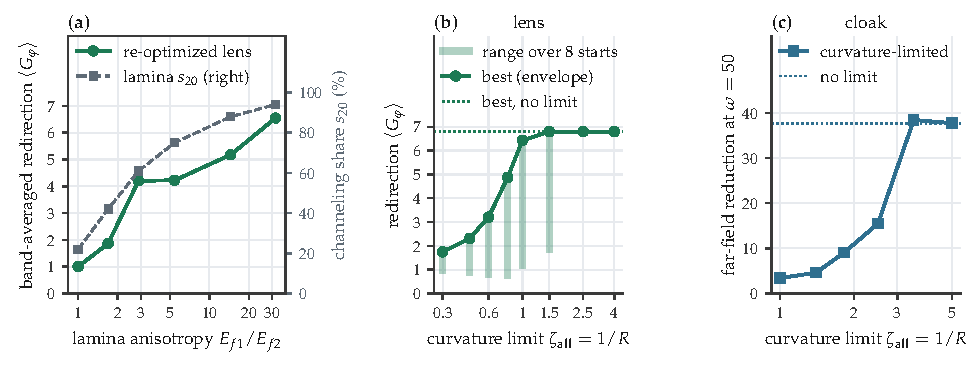
\includegraphics[width=\textwidth]{figs/wt_limits.pdf}}{\fbox{\textit{figure pending}}}
\caption{What bounds orientation control. \textbf{(a)}~Band-averaged redirection of the
re-optimized lens vs.\ lamina anisotropy, with the channeling share $s_{20}$ of the
lamina (right axis; both axes start at zero). \textbf{(b)}~Band-averaged redirection of
the lens and \textbf{(c)}~far-field reduction of the cloak at $\omega=50$ vs.\ the
tow-curvature limit $\zeta_{\rm all}=1/R$ (lengths in the nondimensional units of the
plate). In (b), circles: the best design found at each limit over all computed designs
that satisfy it (a lower bound on what the limit allows); shaded bars: the range over the
independent starts run at that limit; dotted: the best design found with no limit
($\WFrontUnc\times$, from a run at $\zeta_{\rm all}=1.5$). In (c), dotted: the loosest-limit run
of this front study ($\zeta_{\rm all}=5$, achieved $\max|\zeta|=4.5$, i.e.\ effectively
unconstrained; $37.7\times$, while the design of Fig.~\ref{fig:cloak}, $36\times$, is an
independent run of the same problem). At $\zeta_{\rm all}=3.5$
the constrained cloak ($38.4\times$) slightly exceeds the unconstrained one
($37.7\times$): the optimizer is local, and the warm-started constrained run found a
marginally better optimum, so the two are equal within optimizer variability.}
\label{fig:limitsW}
\end{figure}

\subsection{The cloak: what bounded anisotropy can and cannot do (W5)}\label{sec:cloak}
On an $8\times5$ plate at $\omega=50$, a circular traction-free void of radius
$R_V=0.55$ is cut conformally from the mesh. Orientation may change only inside a shell
$r<R_{\rm des}=1.5$ (exactly straight outside, enforced by a smooth taper carried through
the chain rule). The far-field mismatch to the void-free reference is minimized outside
$R_C=1.7$, a region the design cannot touch.
\begin{itemize}[itemsep=1pt]
\item \textbf{At the design frequency.} The optimized shell reduces the mismatch
  $\WCloakPeak\times$ (Fig.~\ref{fig:cloak}). The transformation-cloak prescription
  \cite{pendry2006,norris2008}, imposed as fiber \emph{directions} on our fixed-contrast
  lamina, gives $\WCloakAnalytic\times$, because what it actually requires is a
  diverging \emph{magnitude} of anisotropy, which no lamina has. Its fiber curvature is
  also singular at the rim: the radial map sends straight tows onto curves that wrap the
  void ever more tightly, so no minimum tow radius is respected (its tow paths are not shown; the field in Fig.~\ref{fig:cloak}d is what these directions achieve).
\item \textbf{Mesh sensitivity.} An interference cancellation is sensitive to the
  discrete dispersion of the mesh it was tuned on. Evaluated on a finer conforming mesh
  ($h=0.03$ instead of $0.045$), the same design gives $\WCloakFineEval\times$, while the
  curvature-limited and transformation-direction designs change less
  ($\WCloakCurv\to\WCloakFineCurv\times$, $\WCloakAnalytic\to\WCloakFineTr\times$). Re-optimized on the finer mesh (warm
  start, 80 iterations), the shell reaches $\WCloakFineReopt\times$, and it is just as narrowband
  ($\WCloakFineMinus\times$ and $\WCloakFinePlus\times$ at $\pm5\%$). The capability
  therefore persists under refinement, while any one optimized design is tuned to its
  discretization
  (Appendix~\ref{app:verify}).
\item \textbf{Across frequency.} As W5 predicts, the optimized cloak is narrowband
  (Table~\ref{tab:cloakband}): $\WCloakMinus\times$ at $\omega=47.5$, $\WCloakPlus\times$
  at $52.5$, and $\WCloakForty\times$ at $40$. There it is outperformed by the
  transformation-direction field ($\WCloakAnalyticForty\times$).
\item \textbf{Under a tow-curvature limit.} With the curvature bounded at the void's own
  scale, $\zeta_{\rm all}=1/R_V$, the cloak reaches $\WCloakCurv\times$ at the design
  frequency (an independent run of the curvature front, Fig.~\ref{fig:limitsW}c, gives
  $9.0\times$ at the same limit). This is less peaked but also less narrowband
  ($\WCloakCurvMinus$--$\WCloakCurvPlus\times$ over $\pm5\%$, and at least
  $\WCloakCurvBandMin\times$ over $\omega\in[40,60]$).
\end{itemize}
Bounded-anisotropy cloaking is therefore real but tuned. Manufacturable orientation
fields can cancel a scatterer's far field strongly at a chosen frequency, and only
moderately across a band.

\begin{table}[h]
\centering\small
\caption{Far-field mismatch reduction of three cloak fields across frequency (all on the
same conforming mesh; designs fixed).}\label{tab:cloakband}
\IfFileExists{wt_cloakband_table.tex}{\begin{tabular}{@{}cccc@{}}
\toprule
$\omega$ & optimized & curvature-limited ($1/R_V$) & transformation directions\\ \midrule
40.0 & 1.9 & 3.7 & 4.6\\
45.0 & 2.5 & 2.9 & 1.8\\
47.5 & 7.5 & 6.2 & 2.8\\
\bf 50.0 & \bf 36.2 & \bf 9.6 & \bf 1.9\\
52.5 & 14.9 & 5.7 & 3.9\\
55.0 & 6.4 & 4.6 & 2.6\\
60.0 & 2.7 & 2.9 & 1.1\\
\bottomrule
\end{tabular}
}{\textit{(pending: run in progress)}}
\end{table}

\begin{figure}[h]
\centering
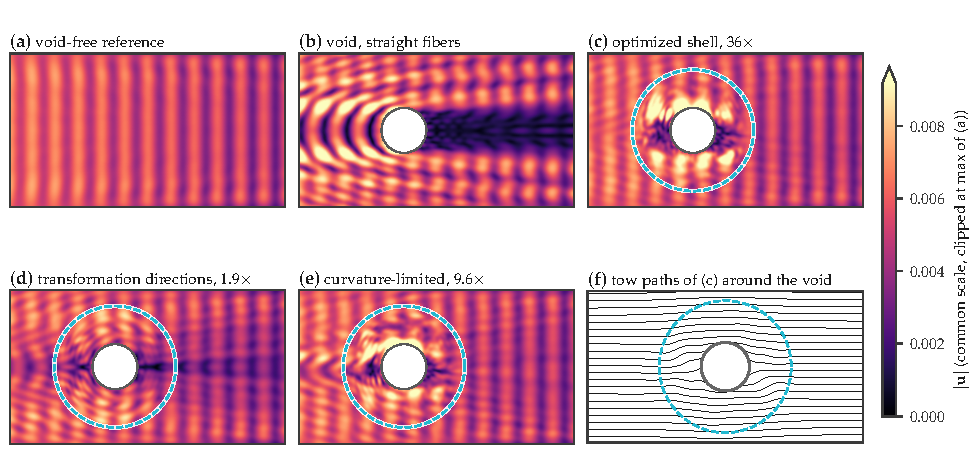
\includegraphics[width=\textwidth]{figs/wt_cloak.pdf}
\caption{Cloaking a conforming traction-free void ($R_V=0.55$) at $\omega=50$, field
magnitude $|\vu|$ (nondimensional) in the plate interior on one common color scale, clipped at the maximum
of the reference (a) (the arrow marks values above it: at most $3.5\%$ of all mesh nodes, near the void, by at
most $1.8\times$). \textbf{(a)}~Void-free
reference. \textbf{(b)}~The void with straight fibers: shadow and reflections.
\textbf{(c)}~Optimized orientation, free only inside the design shell (dashed circle, same in (c)--(f)).
\textbf{(d)}~Transformation-cloak fiber \emph{directions} imposed on the fixed-contrast lamina.
\textbf{(e)}~Optimized under the tow-curvature limit $\zeta_{\rm all}=1/R_V$.
\textbf{(f)}~Tow paths of (c) around the void (same aspect ratio, centered on the void and enlarged by about $7\%$), wrapping the void inside the shell
and straight outside it.
Reductions of the far-field mismatch are given in the panel titles; Table~\ref{tab:cloakband}
shows that the strong reductions are confined to the design frequency, while the
curvature-limited design holds a moderate reduction across the band.}
\label{fig:cloak}\label{fig:cloakh2h}
\end{figure}

\subsection{Design practice: a band-robust multifunctional panel}\label{sec:panel}
The preceding results imply two design rules. Optimize over a frequency band rather
than at one frequency, so that the optimizer cannot buy performance with a resonance.
Ask the fiber field to route energy, which channeling does broadband. A bolted
$7\times4$ CFRP panel with four conforming fastener holes is designed this way. A single
mirror-symmetric, curvature-feasible field ($\max|\zeta|=\WPanZmax\le1/R_{\rm tow}$),
optimized over $\WPanNF$ frequencies in $[\WPanBLo,\WPanBHi]$, does four things at the band center (Fig.~\ref{fig:panel}; parameters in
Table~\ref{tab:panelparams}):
\begin{itemize}[itemsep=1pt]
\item it routes the incident vibration onto a sensor patch ($\WPanRoute\times$);
\item it shields a payload core to $\WPanShield\times$ its straight-fiber energy;
\item it keeps the four fatigue-critical fastener rims at $\WPanProt\times$;
\item it stiffens the bolted mount $\WPanStiff\times$ at no added mass (stiffness is an explicit, weighted term of the objective).
\end{itemize}
Across the band (Fig.~\ref{fig:panel}d) the payload stays at or below
$\WPanBandPayMax\times$ and the rims at or below $\WPanBandRimMax\times$ their straight-fiber
energies, and the sensor stays above its straight-fiber level (lowest
$\WPanBandSenMin\times$ at $\omega=\WPanBandSenMinW$); outside the band it can dip below it
($\WPanBandSenOutMin\times$). A design optimized at the band center alone, with the same
settings, routes slightly better (sensor at least $\WPanToneSenMin\times$ in the band) and
shields better at the band center, but lets the rim protection degrade toward the lower
band edge, to $\WPanToneRimMax\times$ the straight-fiber energy, i.e.\ worse than straight
fibers. The band objective buys robust rim protection at a small cost in routing.
The objective, a single signed region weight with logarithmic delivery and
straight-fiber normalization, is given in Appendix~\ref{app:panelobj}.

\begin{figure}[h]
\centering
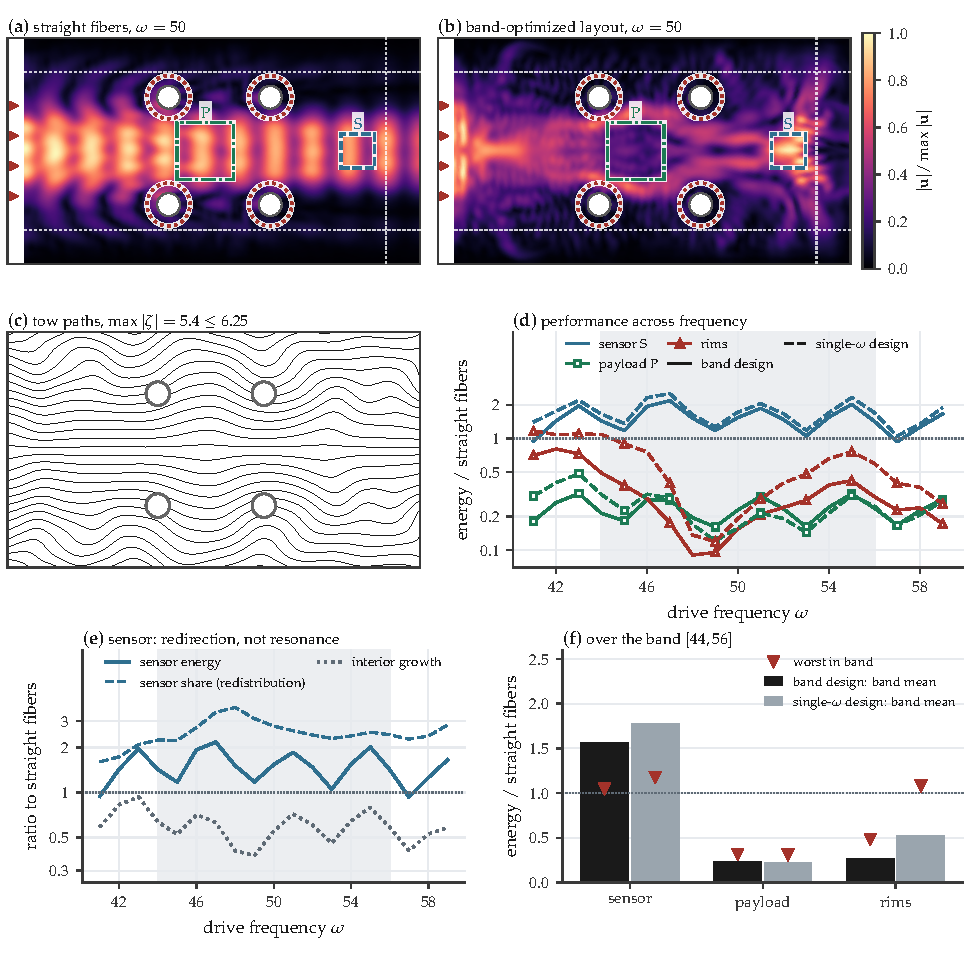
\includegraphics[width=\textwidth]{figs/wt_panel.pdf}
\caption{Band-robust multifunctional panel (four conforming fastener holes; drive at the
left edge). \textbf{(a,b)}~$|\vu|$ at the band center with straight fibers and with the
band-optimized layout, each normalized by its own maximum: the beam splits around the
payload (P, green dash-dot) and reconverges on the sensor (S, blue dashed) while the
fastener rims (red dotted) stay quiet. \textbf{(c)}~Tow
paths, curvature-feasible. \textbf{(d)}~Energy in the sensor, payload and rims relative to
straight fibers across frequency, for the band-optimized design (solid) and a design
optimized at $\omega=50$ only (dashed); shaded: design band; dotted: parity with
straight fibers. The single-frequency design
lets rim protection degrade toward the lower band edge.}
\label{fig:panel}
\end{figure}
